\Subhead{2.2.2}{Волновой пакет в первом и втором приближении. Параболическое уравнение. Расплывание и компрессия импульсов}

В сопутствующем времени $\tau=t-k'_0z$ второе приближение дисперсии даёт
\begin{equation}\label{eq:temporalparabolic}
 \partial_zA=-\frac{\ii k''_0}{2}\partial_\tau^2A.
\end{equation}
Знак следует непосредственно из спектрального множителя $\exp(\ii k''_0z\Omega^2/2)$. Условия: $\Delta\omega\ll\omega_0$, высшие члены $|k_0^{(3)}z(\Delta\omega)^3|\ll1$, поглощение почти постоянно в полосе. Для начального $A(0,\tau)=A_0\exp[-\tau^2/(2T_0^2)]$
\begin{equation}
 A(z,\tau)=\frac{A_0}{\sqrt{1-\ii z/L_D}}
 \exp\left[-\frac{\tau^2}{2T_0^2(1-\ii z/L_D)}\right],\quad
 L_D=\frac{T_0^2}{k''_0}.
\end{equation}
Ширина интенсивности по уровню $1/\e$ равна $T_0\sqrt{1+(k''_0z/T_0^2)^2}$. Энергия пакета сохраняется, максимум уменьшается, возникает частотная модуляция. Знак $k''$ определяет знак модуляции, но незачирпованный пакет расширяется при обоих знаках.

Если исходный спектр имеет фазу $\phi_2\Omega^2/2$, дисперсия добавляет $k''_0z\Omega^2/2$. Компрессия возможна при $\phi_2+k''_0z\simeq0$: задержанные компоненты догоняют ранние. Минимальная длительность ограничена шириной спектра; без расширения полосы нельзя получить произвольно короткий импульс.

Пространственное параболическое уравнение имеет сходную форму. Подстановка $U=A(x,y,z)\e^{\ii kz}$ в уравнение Гельмгольца с отбрасыванием $A_{zz}$ даёт $2\ii kA_z+\Delta_\perp A=0$. Здесь расплывание вызывается угловым спектром, а не временной дисперсией.
\begin{center}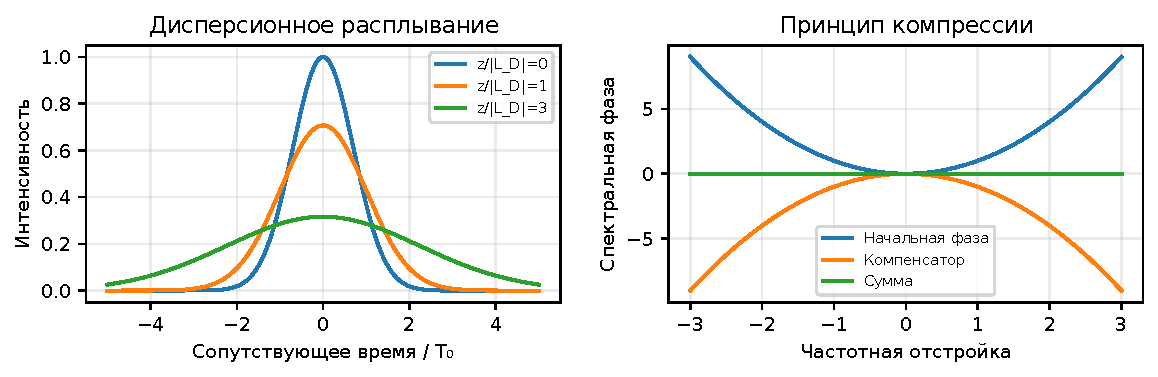
\includegraphics[width=0.8\linewidth]{figures/dispersion.pdf}\end{center}

